\chapter{Thorium Fuel Cycle}

Thorium based nuclear fuel have been of interest from 1950 to 1970 \cite{Th_cycle_viability}. This led to the development of multiple experimental reactors that could operate with thorium based fuel \cite{TMSR_book}. In the 1950, thorium was of special interest due to its higher abundance compared to uranium, being three times more abounded than uranium \cite{Th_cycle_viability,TMSR_book}. Recently, there is a renewed interest in thorium fuel cycle to generate electricity at commercial scale. This renewed interest can be attributed to the multiple factors, some of which are the generation IV reactors based on thorium based nuclear fuel, China and USA research project on thorium utilization for molten salt reactors and the new Atomic Act on Peaceful Utilization of Nuclear Energy and Ionizing Radiation published as Act No. 253/2016 Coll effective since 2017 \cite{Th_cycle_viability}.     

The thorium fuel cycle is based on the use of \(\prescript{232}{}{Th}\) as fertile material, which is converted into fissile \(\prescript{233}{}{U}\) by neutron capture and beta decay. This implies that an additional step of converting the fertile isotope into the fissile material is required. The subsequent use of \(\prescript{233}{}{U}\) as fuel is possible in two ways. The first option is an open fuel cycle, based of the breading of \(\prescript{233}{}{U}\) and in situ fission of this isotope, this would not involve chemical separation of \(\prescript{233}{}{U}\) from the irradiated fuel \cite{IAEA_Th_Potential}. The second option is a closed fuel cycle, where the irradiated fuel is reprocessed to separate the fissile material from the rest of the irradiated fuel, this fissile material is then used to fabricate new fuel elements \cite{IAEA_Th_Potential}. 

\section{Considerations for the Thorium Fuel Cycle}

The chemical properties of thorium make thorium dioxide more stable and has higher radiation resistance than uranium dioxide \cite{IAEA_Th_Potential}. \(ThO_2\) has higher thermal conductivity and lower coefficient of thermal expansion compared to \(UO_2\), this might make \(ThO_2\) based fuels to have a better in-pile perform \cite{IAEA_Th_Potential}. Furthermore, \(ThO_2\) is considered inert and does not oxidize unlike \(UO_2\), making long term storage of irradiated fuel easier \cite{IAEA_Th_Potential}.

The thorium fuel cycle has a higher conversion ratio in thermal reactors compared to the uranium fuel cycle, this is due to the fact that \(\prescript{232}{}{Th}\) has a higher neutron capture cross section compared to \(\prescript{238}{}{U}\) with thermal neutrons \cite{IAEA_Th_Potential}. Additionally, the fraction of neutrons liberated per neutron absorbed (\(\eta\)) is greater than \(2.0\) over a wide range of thermal neutron, unlike \(\prescript{235}{}{U}\) and \(\prescript{239}{}{Pu}\). Making \(\prescript{232}{}{Th} - \prescript{233}{}{U}\) operational with fast or thermal spectra. Unlike \(\prescript{238}{}{U} - \prescript{239}{}{Pu}\) which a breading chain reaction can only be obtained with fast neutrons \cite{IAEA_Th_Potential}.

Finally, the thorium fuel cycle has ``intrinsic proliferation resistance'' \cite{IAEA_Th_Potential}. This is because of the formation of \(\prescript{232}{}{U}\) via neutron multiplication reactions (\(n,2n\)) with \(\prescript{232}{}{Th}, \prescript{233}{}{Pa}\) and \(\prescript{233}{}{U}\). \(\prescript{232}{}{U}\) has physical properties, such as a very short half-life (\(t_{1/2} = 68.90 \, \text{years} \)) and the emission of strong gamma radiation by its decay products \cite{IAEA_Th_Potential,NNDC}. This makes the thorium fuel cycle less attractive for the production of nuclear weapons \cite{IAEA_Th_Potential}.

\section{Thorium Front End}

All thorium isotopes have short half-lives, except \(\prescript{232}{}{Th}\) which has a half-life of \(t_{1/2} = 1.405 \times 10^{10} \, \text{years}\) \cite{NNDC}, making all the natural thorium available on earth constituted by \(\prescript{232}{}{Th}\). Generally, Natural thorium is presented in association with other elements, such as rare earths elements and uranium in diverse rocks types such as veins of thorite, thorianite, uranothorite and  monazite in granite and other acidic intrusions \cite{IAEA_Th_Potential}. 

The global thorium reserves to \(2013\) are estimated to be around \(6.24 \, \text{million tons}\). India has the largest thorium reserves, with approximately \(846,000 \, \text{tons}\), followed by Brazil with \(632,000 \, \text{tons}\) and the United States with \(595,000 \, \text{tons}\) \cite{Th_cycle_viability}.

Thorium reserves in Colombia are associated mainly with igneous rocks, such as granite and pegmatites, and can also be found in placers, especially in alluvial deposits \cite{Th_Colombia}. The concentration of thorium in the country varies significantly depending on the geological formation, with values ranging between \(0.1\) and \(585 \, \text{mg}/\text{kg}\) in sediments. The highest concentrations are observed in areas with granitic formations, such as the Sierra Nevada de Santa Marta and parts of the Andean region, which are known for their igneous and metamorphic rocks \cite{Th_Colombia}. 

The mining and extraction of thorium from monazite is relatively straightforward and differs significantly from the extraction of uranium from its ores. Most commercially exploited monazite comes from beach or river sands, often alongside other heavy minerals. Compared to uranium mining, thorium extraction involves much less overburden, and the radioactive waste produced is approximately two orders of magnitude lower. The so-called radon impact is also considerably smaller for thorium mining, due to the shorter half-life of thoron (\(\prescript{220}{}{Rn}\)) compared to radon (\(\prescript{222}{}{Rn}\)), leading to simpler tailings' management \cite{IAEA_Th_Potential,Thoron}.

The monazite is finely ground and dissolved in concentrated sodium hydroxide at around \(140^{\circ}C\), followed by a series of chemical processes, including solvent extraction and ion exchange, to yield pure thorium nitrate. This is then precipitated as thorium oxalate and calcined to obtain \(ThO_2\) powder. Thorium recovery projects typically separate thorium in pure oxalate form, which is easier to handle and store for future applications, such as preparing mantle-grade thorium nitrate or nuclear-grade thorium oxide. Uranium present in monazite is also separated in the form of crude uranium concentrate during the process \cite{IAEA_Th_Potential}.

\section{Thorium Open Fuel Cycle}

An open fuel cycle avoids the complex engineering requirements associated with reprocessing irradiated fuel and fabricating highly radiotoxic \(\prescript{233}{}{U}\)-based fuels. The core layout is designed such that each fuel assembly comprises a ``seed'' material, typically medium-enriched uranium or plutonium, and ``blanket'' material of thorium \cite{IAEA_Th_Potential}. Separation of seed and blanket, optimization moderator to fuel ratio and long periods of fuel usage offer the possibility that around \(40 \, \%\) of the power generated by fission comes from \(\prescript{233}{}{U}\) \cite{IAEA_Th_Potential}.

This scheme is very attractive for an introduction if thorium in nuclear power reactors because of the direct utilization of \(\prescript{233}{}{U}\), avoiding the need of reprocessing and fabrication of new fuel elements with \(\prescript{233}{}{U}\) \cite{IAEA_Th_Potential}. Furthermore, the once-through thorium fuel cycle opens the possibility of incineration if weapons-grade plutonium in light water reactors \cite{IAEA_Th_Potential}. To achieve this, thorium oxide containing \(5 \, \%\) of \(PuO_2\), could be used as driver fuel. The exclusion of uranium from the fuel composition results in an increase in the rate of plutonium incineration compared to standard MOX fuel \cite{IAEA_Th_Potential}.

Similarly, civil plutonium could be burned in a thorium fuel cycle by using the same combination of thorium oxide and plutonium oxide \cite{IAEA_Th_Potential}. Since, \(\prescript{240}{}{Pu}\) is present is significant quantities in civil grade plutonium, and it is a good burnable absorbed, then there is no need for use burnable absorber in the form of gadolinium, integrated into the fuel \cite{IAEA_Th_Potential}. Plutonium oxide fuel without major modification in the reactor core could be a direct replacement for LEU oxide fuel \cite{IAEA_Th_Potential}.

\section{Thorium Closed Fuel Cycle}

The closed fuel cycle for thorium-based fuels includes essential steps such as reprocessing irradiated fuel and separating converted \(\prescript{233}{}{U}\). In some reactor designs, like LWRs, mixed thorium-plutonium oxide fuel is used to facilitate the conversion of \(\prescript{232}{}{Th}\) to \(\prescript{233}{}{U}\). However, an important consideration in recycling \(\prescript{233}{}{U}\) is the presence of \(\prescript{232}{}{U}\), which introduces radiological challenges due to its strong gamma emissions \cite{IAEA_Th_Potential}.

Various countries have implemented closed thorium fuel cycles. In Russia, fast breeder reactors like the BN-800 have been studied for their capability to achieve self-sufficiency in the \(\prescript{232}{}{Th}-\prescript{233}{}{U}\) cycle with a breeding ratio close to or exceeding 1.0. France has also explored similar concepts in reactor types such as high-temperature gas-cooled reactors (HTGRs) and HWRs, finding that these reactors can approach a breeding ratio of 1.0, though not exceed it \cite{IAEA_Th_Potential}.

India has adopted a strategic three-stage nuclear program to maximize its vast thorium reserves. The first stage, utilizing PHWRs, employs \(\text{ThO}_2\) assemblies to flatten neutron flux. The second stage, using liquid metal-cooled fast breeder reactors (LMFBRs), incorporates \(\text{ThO}_2\) blankets to produce \(\prescript{233}{}{U}\). Finally, the third stage involves advanced thermal reactors that are self-sustaining in \(\prescript{232}{}{Th}-\prescript{233}{}{U}\) fuels, like the Advanced Heavy Water Reactor (AHWR) designed by Bhabha Atomic Research Center (BARC). This multistage program enables India to establish a sustainable thorium cycle by gradually transitioning to a thorium-based closed fuel cycle \cite{IAEA_Th_Potential}.

\subsection{Reprocessing}

The THOREX (Thorium-uranium EXtraction) process is the primary method proposed for reprocessing thorium-based fuels. Developed at Oak Ridge National Laboratory in the 1950s, THOREX uses solvent extraction with tributyl phosphate (TBP) to separate uranium and thorium from fission products. This process builds on the success of TBP in the PUREX process, making it a natural choice for thorium fuel reprocessing. The THOREX process has mainly been implemented at laboratory or pilot scales in a few countries. For example, India established a facility at BARC in 1970 to reprocess thorium irradiated in the CIRUS reactor (Canada India Reactor Utility Services), successfully achieving high-purity \(\prescript{233}{}{U}\) with minimal \(\prescript{232}{}{U}\) contamination \cite{IAEA_Th_Potential,fuel_cycle_book}.

The objective of the THOREX process is to separate and purify \(\prescript{232}{}{Th}\), \(\prescript{233}{}{U}\), and \(\prescript{233}{}{Pa}\) from irradiated thorium fuel, effectively minimizing impurities and contaminants. Despite its technical feasibility, the process has yet to reach the commercial maturity of PUREX, primarily due to engineering challenges such as solvent handling and multiple purification stages. Current research has led to the development of three primary THOREX flowsheets: Interim 23, THOREX-1, and THOREX-2, each offering distinct methods for optimizing separation and improving the efficiency of thorium fuel reprocessing \cite{fuel_cycle_book}.

\subsubsection{Interim 23}

Developed to recover \(\prescript{233}{}{U}\) from irradiated thorium fuel, the Interim 23 process uses \(1.5 \, \%\) TBP in solutions of irradiated thoria (\(ThO_2\)). In this process, silica gel is applied to remove protactinium (\(Pa\)), while Dowex 50 exchange resin is used to concentrate the final product. The process achieves a thorium separation factor of over \(10^5\) with an overall loss of approximately \(0.5\%\). Additionally, solvent extraction provides a fission product separation factor of greater than \(10^5\), which improves to \(10^7\) after the silica gel and concentration steps \cite{fuel_cycle_book}.


\subsubsection{THOREX-1}

The THOREX-1 process was developed with the aim of separating \(\prescript{233}{}{Pa}\), \(\prescript{233}{}{U}\), and \(\prescript{232}{}{Th}\) from irradiated thorium fuel. The process involved multiple stages: diisobutyl carbitol was used specifically for the separation of \(\prescript{233}{}{Pa}\), \(\prescript{233}{}{U}\) extraction was performed with \(5 \, \%\) TBP, and \(\prescript{232}{}{Th}\) extraction required a higher concentration of \(45 \, \%\) TBP. Although the THOREX-1 process achieved adequate decontamination of the products, it encountered significant engineering challenges. These included the complexity of handling different solvents, separate chemical treatments for solvent purification, and managing hot solutions across various processing stages \cite{fuel_cycle_book}.


\subsubsection{THOREX-2}

An alternative TBP-based process for separating \(\prescript{233}{}{U}\) and thorium from irradiated thorium fuel has been developed. This method uses a single TBP solvent system with concentrations between \(41 \, \%\) and \(55 \, \%\) for the initial separation of thorium and uranium. The process begins under slightly acidic conditions, intentionally kept low to minimize the extraction of protactinium and fission products while avoiding thorium precipitation. To ensure Pa remains in the high-active waste stream, an aluminum nitrate scrub solution is added, maintaining a mildly acidic environment. Separation of thorium from uranium is achieved through selective stripping with dilute nitric acid, and \(\prescript{233}{}{U}\) is removed using a very low-concentration nitric acid solution \cite{fuel_cycle_book}. 

Careful regulation of flow rates is necessary to prevent third-phase formation, which can complicate thorium separation. This approach avoids the need for benzene as a solvent. Following this, Pa is recovered by adsorption onto a silica gel column, eliminating the need for further adjustments to the feed solution. By adjusting acidity levels and controlling flow rates at each stage, the process maintains effective separation of \(\prescript{233}{}{U}\) and thorium with minimal loss \cite{fuel_cycle_book}.

\subsection{Backend Issues}

The backend of the thorium fuel cycle presents unique challenges that must be addressed before thorium can be widely adopted in commercial reactors. Key issues include the management of radionuclide inventories in spent thorium-based fuels, which may contain various fertile/fissile combinations, such as \(\prescript{232}{}{Th}-\prescript{235}{}{U}-\prescript{238}{}{U}\), \(\prescript{232}{}{Th}-\prescript{239}{}{Pu}\), and \(\prescript{232}{}{Th}-\prescript{233}{}{U}\). An understanding of the residual heat, radiological impact, and quantities of actinides and long-lived fission products in these spent fuels is essential \cite{IAEA_Th_Potential}.

Several additional challenges complicate the reprocessing of thorium-based fuels. Protactinium (\(\prescript{233}{}{Pa}\)), formed as an intermediate in the conversion of \(\prescript{232}{}{Th}\) to \(\prescript{233}{}{U}\), has a relatively long half-life (27 days) compared to \(\prescript{239}{}{Np}\) in the uranium cycle. This requires a cooling period of around 12 months to allow \(\prescript{233}{}{Pa}\) to decay to \(\prescript{233}{}{U}\), avoiding loss of fissile material. Protactinium, often relegated to the waste stream, also introduces radiological concerns due to \(\prescript{231}{}{Pa}\), a long-lived alpha emitter in the thorium chain. Attempts to co-extract Pa with U and Th in the \(HNO_3–TBP/\text{kerosene}\) process have been unsuccessful, though a selective adsorption technique using Vycor glass has shown promise, achieving approximately \(98 \, \%\) separation of protactinium \cite{IAEA_Th_Potential}.

The presence of \(\prescript{232}{}{U}\) in spent thorium fuel is another concern. \(\prescript{232}{}{U}\), formed through neutron interactions with \(\prescript{232}{}{Th}\) and its products, decays into gamma-emitting daughters like \(\prescript{208}{}{Tl}\), complicating handling and storage due to the high radiation levels. The \(\prescript{232}{}{U}\) content is influenced by the neutron spectrum and irradiation duration, with fast reactors yielding higher \(\prescript{232}{}{U}\) levels than thermal reactors. Strategies such as positioning thorium blankets away from the core in reactors like the BN-350 have successfully minimized \(\prescript{232}{}{U}\) concentrations in the produced \(\prescript{233}{}{U}\).

Lastly, dissolving thorium dioxide in nitric acid presents challenges, as \(ThO_2\) is highly stable compared to uranium and plutonium oxides. Dissolution generally requires the addition of hydrofluoric acid (HF) to nitric acid, though this accelerates corrosion of processing equipment. The THOREX reagent is the most effective solution developed to date for dissolving Th-based fuels. Higher temperatures and pressures during dissolution also improve the process, addressing this unique aspect of thorium reprocessing \cite{IAEA_Th_Potential}.

\section{Molten Salt Reactors (MSR)}

Currently, most nuclear power plants operate with LWRs, which present several disadvantages. One key issue is the proliferation risk due to the production of \(\prescript{239}{}{Pu}\) in used fuel, which remains a concern whether the fuel is reprocessed or disposed of as waste. Additionally, LWRs have limited thermal efficiency, typically capped at around \(35\,\%\), due to temperature constraints. There is also the risk of steam explosions in these reactors, as well as high core after heat during accidents, which raises the danger of fuel melting, as observed in incidents like Three Mile Island and Fukushima \cite{TMSR_book}.

MSRs offer promising solutions to many of these challenges. Unlike LWRs, MSRs can operate at low pressures, reducing the risks associated with high-pressure containment and the need for robust, large containment domes. Moreover, MSRs eliminate the need for cladding, which reduces the risk of cladding failure and hydrogen production, a key contributor to explosions in accidents involving high-temperature interactions between zirconium cladding and water. Since the fuel in an MSR is already molten, there is no risk of solid fuel melting during accidents \cite{TMSR_book}.

In addition, MSRs provide advantages such as continuous online refueling and reactivity adjustments, which allow for smoother operation and safer control. They can also maintain lower core excess reactivity, simplifying reactor control. Continuous removal of fission products, such as \(\prescript{137}{}{Cs}\), reduces core radioactivity and mitigates the release of contaminants in severe accidents. Noble gases like xenon and krypton, which cause xenon poisoning in reactors, can be easily removed, avoiding common control issues seen in LWRs \cite{TMSR_book}.

\subsection{Challenges for the Implementation of Molten Salt Reactors}

Several issues should be addressed before implementing an MSR. One challenge is that the fuel flowing out of the reactor continues to emit radiation, requiring a remote maintenance required for the plumbing. Other limiting factor is the corrosion of structure and plumbing materials, which must withstand the high temperatures and corrosive environment of the molten salt, this could be alleviated using Hastelloy-N, a nickel-based alloy that has shown good resistance to corrosion in molten salt environments \cite{TMSR_book,Haynes2024}.

Another challenge is the need for a reprocessing facility to separate fission products and actinides from the fuel salt. This facility must be able to handle the high radiation levels of the fuel salt, which can be achieved by using remote maintenance and shielding. The reprocessing facility must also be able to separate the fission products and actinides from the fuel salt, which can be achieved using solvent extraction \cite{TMSR_book}.

\subsection{Thorium Molten Salt Reactors}

The thorium molten salt reactor (TMSR) is designed for thorium based nuclear energy utilization. There are two possible implementations of TMSRs: the liquid-fueled (TMSR-LF) and the solid-fueled (TMSR-SF) \cite{TMSR_book}.

\subsubsection{Liquid Fuel Thorium Molten Salt Reactor (TMSR-LF)}

The TMSR-LF is designed to produce an electrical power output of 168 MWe per unit and can be scaled to meet different power needs, including configurations of one, two, or six units, reaching up to GWe. This reactor consists of three main loops: the primary loop with fuel salt, a secondary loop for isolating radioactivity, and a third loop for energy utilization. In the primary loop, a molten salt mixture of \(LiF-BeF_2-UF_4-ThF_4\) is used, where the lithium is enriched to \(99.995 \, \%\) in \(\prescript{7}{}{Li}\) and uranium to \(19.75 \, \%\) in \(\prescript{235}{}{U}\). The secondary loop contains FNaBe salt. The inlet and outlet temperatures of the primary loop are \(600^{\circ}C\) and \(700^{\circ}C\), respectively, allowing high-efficiency power generation through a combined Brayton and Rankine cycle, achieving thermoelectric conversion efficiencies above \(45 \, \%\) \cite{TMSR_book}.

The TMSR-LF features an online refueling system that maintains low excess reactivity, along with an off-gas system to continuously remove gaseous fission products, including xenon, helium, and tritium. This improves neutron economy and reduces the demands on the reactivity control system. For safety, a passive residual heat removal system is designed to manage heat during accident scenarios, and a passive fuel salt discharge system with a freezing valve is incorporated to safely shut down and dissipate heat under extreme conditions \cite{TMSR_book}.

The TMSR-LF plant layout is divided into three main zones: the nuclear island, conventional island, and service region. The nuclear island, housing key nuclear components, is located underground to enhance safety, while the conventional island, containing auxiliary facilities like cooling towers and turbines, is placed nearby to reduce heat transfer distances. Additional auxiliary buildings, including those for hydrogen production and seawater desalination, are part of the conventional island \cite{TMSR_book}. This schematic is represented in \textbf{Fig.} \ref{fig:TMSR-LF}.

\begin{figure}[h]
    \centering
    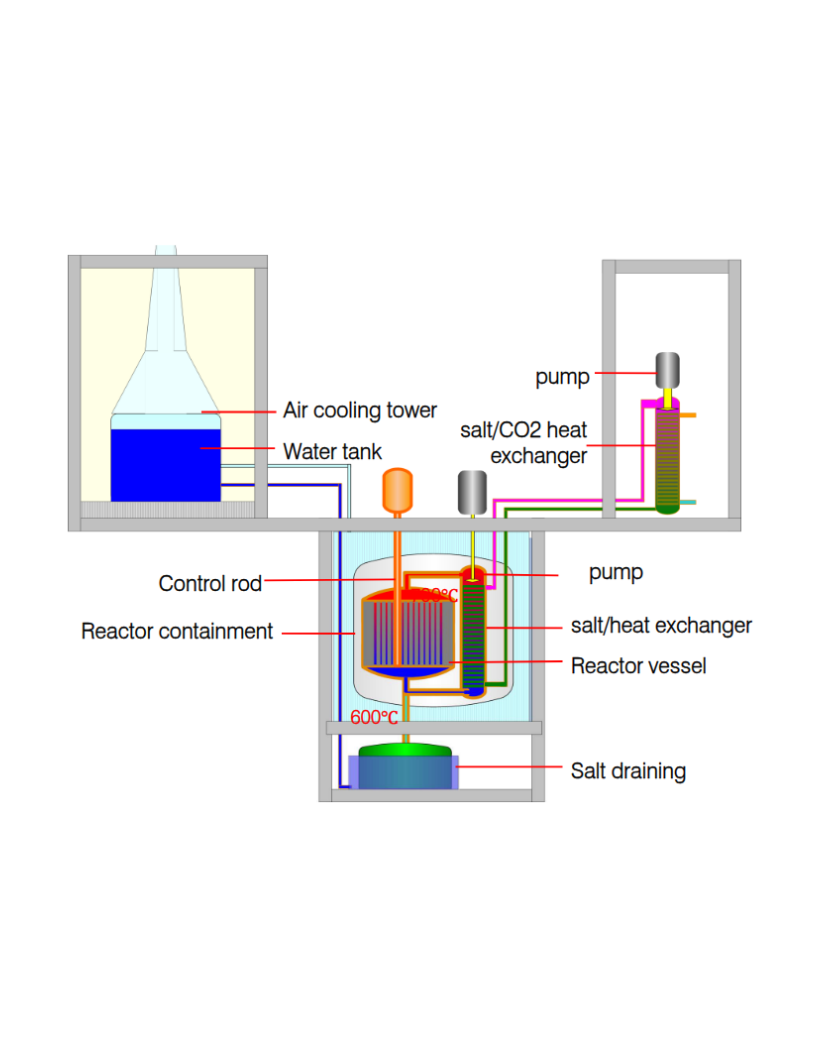
\includegraphics[scale=0.5]{Kap6/Figures_Kap6/TMSR-LF_2.png}
    \caption{Liquid Fuel Thorium Molten Salt Reactor (TMSR-LF) design. From \textbf{Ref.} \cite{Xu2017}}
    \label{fig:TMSR-LF}    
\end{figure}

Designed with modularity in mind, the reactor body module of the TMSR-LF has a lifespan of approximately five years, with easy installation and replacement. The reactor vessel and primary circuit are housed within a steel containment structure, which acts as an additional safety barrier. A gas layer between the containment and reactor vessel also aids in tritium removal. The TMSR-LF is a promising candidate for implementing the \(Th-U\) fuel cycle, aiming to optimize thorium resource use, reduce nuclear waste, support nonproliferation efforts, and ultimately achieve a fully closed \(Th-U\) cycle \cite{TMSR_book}.

\subsubsection{Solid Fuel Thorium Molten Salt Reactor (TMSR-SF)}

The TMSR-SF is a small modular fluoride salt-cooled high-temperature reactor (FHR) with an electrical power output comparable to the TMSR-LF. These nuclear systems use TRISO (Tristructural-Isotropic) fuel, where each fuel particle has a uranium dioxide (\(\text{UO}_2\)) kernel surrounded by a multi-layered coating. This coating consists of a low-density carbon buffer layer that accommodates fission gases, a silicon carbide (SiC) layer to act as a primary barrier for fission products, and two high-density isotropic pyrolytic carbon (PyC) layers encasing the SiC \cite{TRISO, IAEA_TRISO_REPORT}. \textbf{Fig.} \ref{fig:TRISO} shows the structure of a TRISO particle.

\begin{figure}[h]
    \centering
    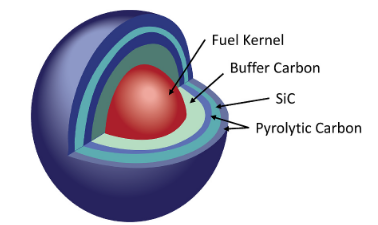
\includegraphics[scale=0.5]{Kap6/Figures_Kap6/TRISO_particle.png}
    \caption{TRISO particle structure. From \textbf{Ref.} \cite{IAEA_TRISO_REPORT}}
    \label{fig:TRISO}
\end{figure}

In the TMSR-SF design, the fuel pebbles are 30-mm diameter spherical elements containing TRISO particles dispersed within a graphite matrix. Each pebble houses approximately 2,400 microfuel particles with uranium kernels enriched to \(19.75 \, \%\). When the reactor core is fully loaded, it contains around \(870,000\) fuel pebbles, packed randomly to optimize neutron distribution. A sophisticated fuel handling system circulates the pebbles through various functions, including loading, discharge, purification, monitoring, and storage, using a combination of mechanical operations, buoyancy, and gravity \cite{TMSR_book}.

Reactivity control is maintained by a dual shutdown system. The primary system includes 12 control rods with rectangular shapes, which move vertically within channels in a SiC plate, while the secondary system consists of eight shutdown blades that can be inserted directly through the graphite reflector into the pebble bed during emergency shutdowns. Both the rods and blades contain natural boron carbide encased in a nickel-based alloy, ensuring they can achieve sufficient shutdown margins to maintain subcritical conditions when needed \cite{TMSR_book}.

Heat management within the TMSR-SF is achieved through salt/air heat exchangers in the secondary loops. These heat exchangers transfer heat from the salt to compressed air in the power conversion unit (PCU) using spirally fluted tube-shell designs, which enhance convective heat transfer. This system can also handle the significant pressure differences between the salt and air sides under normal operating conditions. The TMSR-SF generates electricity using an open-air Brayton cycle combined with a steam Rankine cycle, achieving thermoelectric conversion efficiencies over \(45 \, \%\). The PCU includes components such as compressors, turbines, generators, and residual heat recovery units. Purified, hot compressed air from the heat exchangers drives turbines for electricity production, while the remaining residual heat powers the steam Rankine cycle to further enhance efficiency \cite{TMSR_book}.

The modular design of the TMSR-SF facilitates efficient installation and maintenance, and its inherent passive safety features enhance operational safety and flexibility. This design approach, along with an underground nuclear island setup, online refueling capabilities, and auxiliary applications such as hydrogen production or seawater desalination, makes the TMSR-SF a versatile and safe option for future thorium-based energy production \cite{TMSR_book}. \textbf{Fig.} \ref{fig:TMSR-SF} shows the TMSR-SF design. 

\begin{figure}[h]
    \centering
    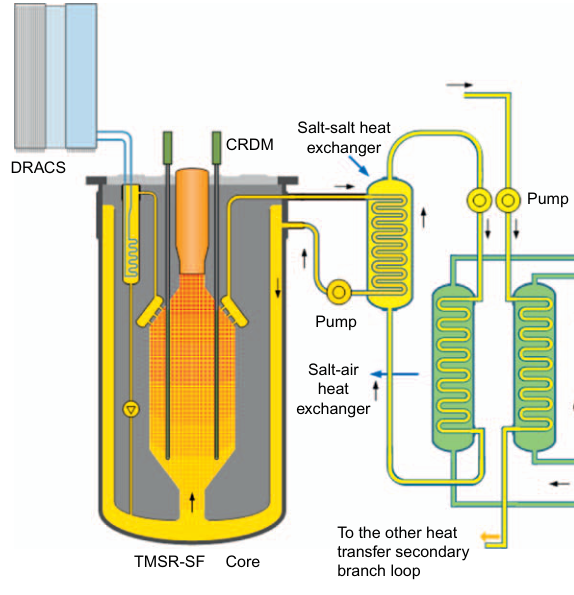
\includegraphics[scale=0.5]{Kap6/Figures_Kap6/TMSR-SF.png}
    \caption{Solid Fuel Thorium Molten Salt Reactor (TMSR-SF) design. From \textbf{Ref.} \cite{TMSR_book}}
    \label{fig:TMSR-SF}
\end{figure}

Having talked about the thorium fuel cycle and the molten salt reactors, the next chapter delve in the simulation of the performance of MOX in a PWR. This is done to understand the behavior of the fuel and the reactor.